\chapter{Paths in Graphs}
\section{Connectivity}
Imagine you are developing a game, where the map is generated automatocally.
In this gate there are several areas connected by portals. So you need to check
that all the areas in your map are reachable from one another.

First we need to somehow understand what we mean by ``reachable'', we say that
an area $A$ is reachable from an area $B$ if there is a path from $A$ to
$B$. To formalize this notion using graphs we need to intrduce a graph
corresponding to the map, consider a graph $G = (V, E)$ such that vertices of
the graph are areas in your map and $(A, B) \in E$ iff the areas $A$ and $B$
are connected by a portal. So a path from $A$ to $B$ is a sequence of areas
$A = C_1$, \dots, $C_\ell = B$ such that $C_i$ and $C_{i + 1}$ are connected by
a portal (i.e. $(C_i, C_{i + 1}) \in E$).
\begin{definition}
  Let $G = (V, E)$ be a graph. We say that a path from $u$ to $v$ is
  a sequence $w_1, \dots, w_\ell \in V$\footnote{%
    Usually such an object is called a walk, and it is called a path if
    all the vertices $w_1$, \dots, $w_\ell$ are different. However,
    for our applications it does not matter and we will use the word ``path''.
  } such that
  \begin{itemize}
    \item $w_1 = u$, $w_\ell = v$, and
    \item $(w_i, w_{i + 1}) \in E$ for $i \in [\ell - 1]$.
  \end{itemize}

  We say that $u, v \in V$ are connected iff there is a path from $u$ to $v$.
  So the graph is connected iff any $u, v \in V$ are connected.
\end{definition}
So, using this notatation, we need to check whether the graph corresponding to
the map is connected.

There are numerous ways to do it, we consider a simple algorithm just to see how
it works.
\begin{algorithm}
  \begin{algorithmic}[1]
    \Function{Connected}{$n$, $E$}
      \State $S \gets \emptyset$
      \State $Q \gets \set{1}$

      \While{$Q \neq \emptyset$}
        \State Choose an element $v$ from $Q$
        \State $Q \gets S \setminus \set{v}$

        \State $S \gets S \cup \set{v}$

        \State $Q \gets Q \cup
          \set[{(v, u) \in E \text{ and } u \notin S}]{u \in [n]}$
      \EndWhile
      \label{line:connectivity-last}
      \State \Return{$S = [n]$}
    \EndFunction
  \end{algorithmic}
  \caption{An algorithm checking whether the graph on $[n]$ with the set of
  edges $E$ is connected.}
  \label{algorithm:connectivity}
\end{algorithm}

\begin{theorem}
  Algorithm~\ref{algorithm:connectivity} checks whether the graph $([n], E)$
  is connected.
\end{theorem}
\begin{proof}
  To prove this we prove that $S$ is equal to the maximal connected subset $U$
  of $[n]$ containing $1$ (we say that a set $U$ is connected iff $G[U]$ is
  connected).

  It is easy to see that $S \subseteq U$.
  Assume that $U \neq S$ on line~\ref{line:connectivity-last}.
  Let $u \in U \setminus S$. Consider a sequence $N_i$ such that
  $N_0 = \set{u}$ and $N_{i + 1} = \set[{u \in N_i, (u, v) \in E}]{v \in [n]}$.
  Note that if a vertex $w \notin S$ on line~\ref{line:connectivity-last}, then
  all the neighbours of $w$ are not $S$. It is also clear that $N_{n} = U$.
  Therefore $S = \emptyset$ which is a contradiction.
\end{proof}

\section{Eulerian Paths}

Graph theory originated from a simple question asked by Leonard Euler:
``Is it possible to walk through the town of K\"{o}nigsberg, starting and
ending at the same place, so that we use each bridge exactly once?'' (the map of K\"{o}nigsberg is depicted on Figure~\ref{figure:konigsberg}).
\begin{figure}
  \begin{center}
    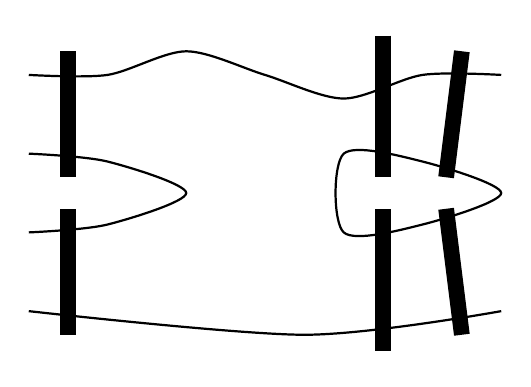
\begin{tikzpicture}[thick]
      \draw plot [smooth] coordinates {(0,0) (1, 0) (2,0.3) (3,0) (4,-0.3) (5, 0) (6, 0)};
      \draw plot [smooth] coordinates {(0, -3) (3.5, -3.3) (6, -3)};

      \draw plot [smooth] coordinates {(0,-1) (1, -1.1) (2, -1.5) (1, -1.9) (0,-2)};

      \draw plot [smooth cycle] coordinates {(4, -1) (5, -1.1) (6, -1.5) (5, -1.9) (4, -2)};

      \draw [line width=2mm] (0.5, 0.3) -- (0.5, -1.3);
      \draw [line width=2mm] (0.5, -3.3) -- (0.5, -1.7);
      \draw [line width=2mm] (4.5, 0.5) -- (4.5, -1.3);
      \draw [line width=2mm] (4.5, -3.5) -- (4.5, -1.7);
      \draw [line width=2mm] (5.5, 0.3) -- (5.3, -1.3);
      \draw [line width=2mm] (5.5, -3.3) -- (5.3, -1.7);
    \end{tikzpicture}
  \end{center}
  \caption{K\"{o}nigsberg's map}
  \label{figure:konigsberg}
\end{figure}

\section{Hameltonian Paths}
